% article example for classicthesis.sty
\documentclass[10pt,a4paper]{article} % KOMA-Script article scrartcl
\usepackage{import}
\usepackage{xifthen}
\usepackage{pdfpages}
\usepackage{transparent}
\newcommand{\incfig}[1]{%
    \def\svgwidth{\columnwidth}
    \import{./figures/}{#1.pdf_tex}
}
\usepackage{lipsum}     %lorem ipsum text
\usepackage{titlesec}   %Section settings
\usepackage{titling}    %Title settings
\usepackage[margin=10em]{geometry}  %Adjusting margins
\usepackage{setspace}
\usepackage{listings}
\usepackage{amsmath}    %Display equations options
\usepackage{amssymb}    %More symbols
\usepackage{xcolor}     %Color settings
\usepackage{pagecolor}
\usepackage{mdframed}
\usepackage[spanish]{babel}
\usepackage[utf8]{inputenc}
\usepackage{longtable}
\usepackage{multicol}
\usepackage{graphicx}
\graphicspath{ {./Images/} }
\setlength{\columnsep}{1cm}

% ====| color de la pagina y del fondo |==== %
\pagecolor{white}
\color{black}



\begin{document}
    %========================{TITLE}====================%
    \title{{  Respuestas Parcial 2 Teoría de Grafos  }}
    \author{{Rodrigo Castillo}}
    \date{\today}

    \maketitle


    %=======================NOTES GOES HERE===================%
    \newpage
    \section{Punto1}
    \textbf{a}:
    \\
    \begin{figure}[h!]
        \centering
        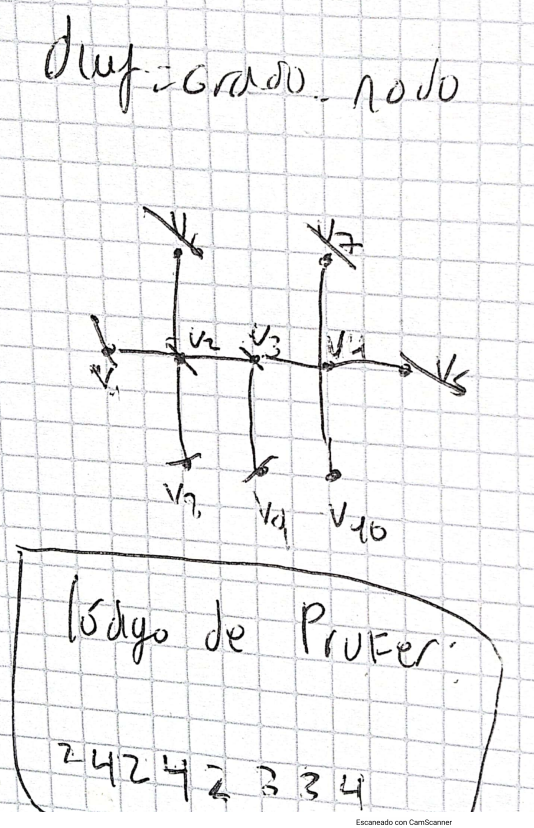
\includegraphics[width=0.4\linewidth]{prufer.png}
        \caption{Código de prufer del arbol dado}
        \label{fig}
    \end{figure}
    \textbf{b:}
    \\
    Arbol generado del código de prufer dado:
    \\
    % ====|ACA EMPIEZA EL PUNTO 1-b|====
    código: $1132435652$
    arbol:
    \\
\begin{figure}[ht]
    \centering
    \incfig{arbolprufer}
    \caption{arbolprufer}
    \label{fig:arbolprufer}
\end{figure}




    % ====|ACA TERMINA EL PUNTO 1-b|==== %


    \newpage
    \section{Punto2}
        \textbf{a:Arbol de expansion mínima encontrado usando el algoritmo de prim:}
        \\
            \begin{figure}[ht]
                \centering
                \incfig{expminima}
                \caption{Arbol de expansión mínima:}
                \label{fig:expminima}
            \end{figure}
            \begin{figure}[h!]
                \centering
                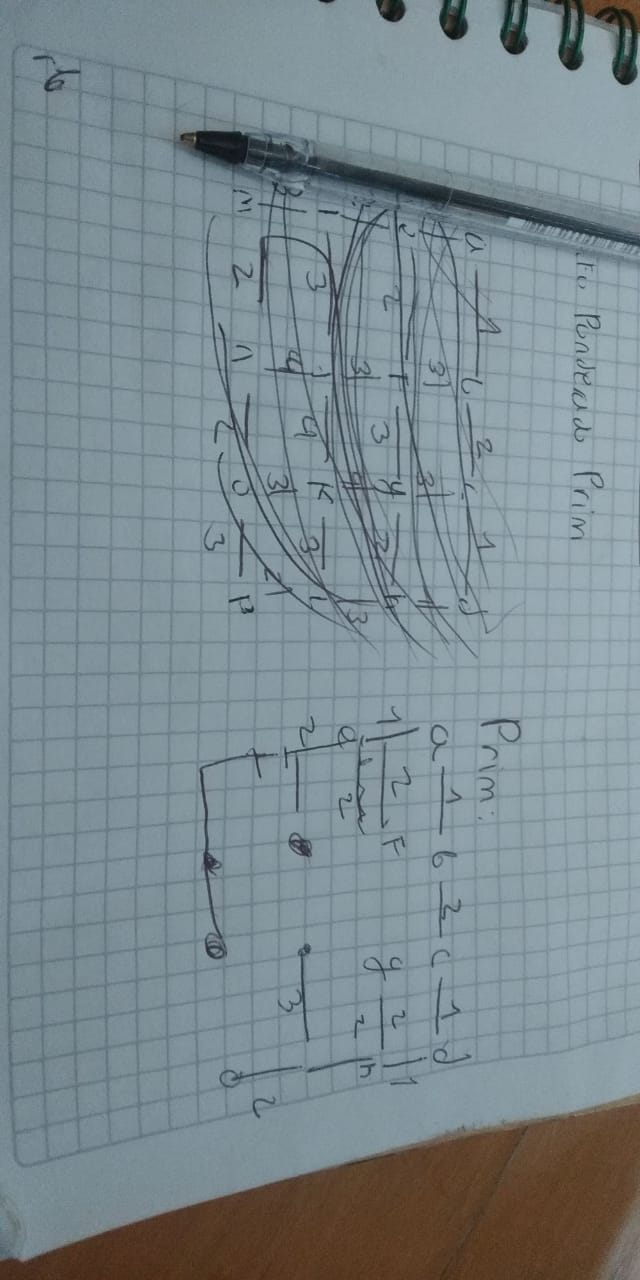
\includegraphics[width=0.4\linewidth]{proc2.jpeg}
                \caption{procedimiento}
                \label{fig}
            \end{figure}




        % ====|ACA TERMINA EL PUNTO  arbol de expansion minima|==== %
        \newpage
        \textbf{b:Arbol de expansión máxima usando kruskal:}
        \\
            \begin{figure}[ht]
                \centering
                \incfig{kruskal}
                \caption{kruskal}
                \label{fig:kruskal}
            \end{figure}

            \begin{figure}[h!]
                \centering
                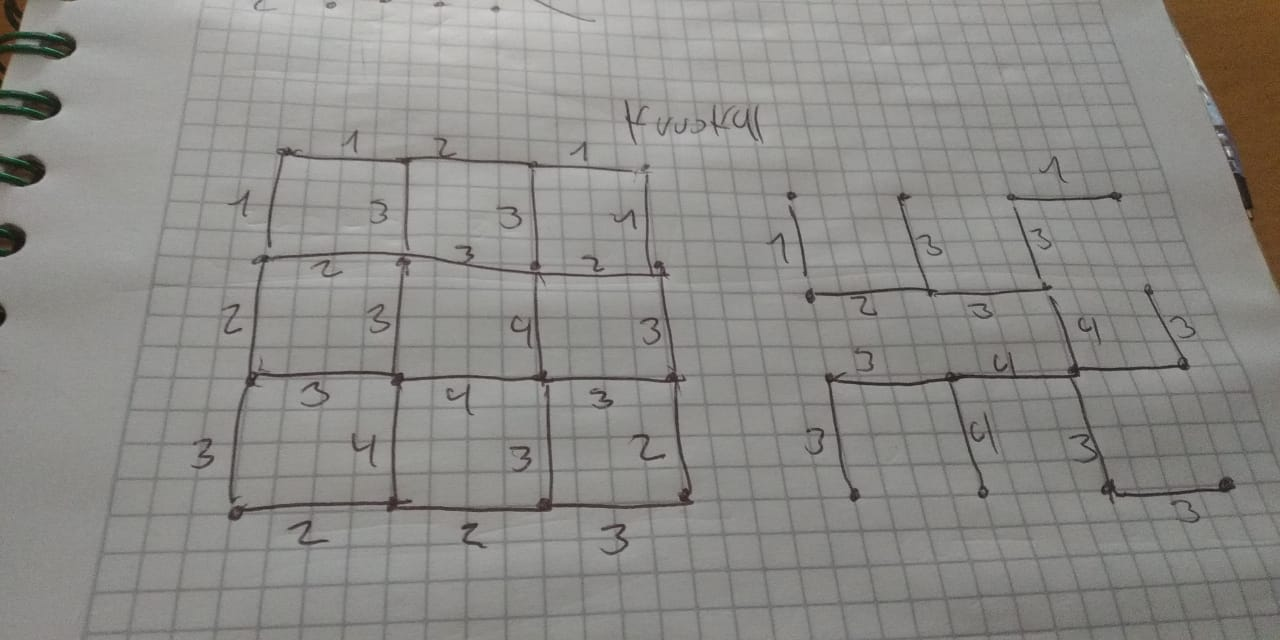
\includegraphics[width=0.8\linewidth]{kruskal.jpeg}
                \caption{Procedimiento kruskal}
                \label{fig}
            \end{figure}




        % ====|ACA TERMINA EL PUNTO Kruskal|==== %
        \textbf{camino minimo entre m y g usando Dijkstra:}
        \\
        % ====|ACA EMPIEZA EL PUNTO Dijkstra|====
            \begin{figure}[ht]
                \centering
                \incfig{rutaminima}
                \caption{Resultado de Dijkstra}
                \label{fig:rutaminima}
            \end{figure}
            \begin{figure}[h!]
                \centering
                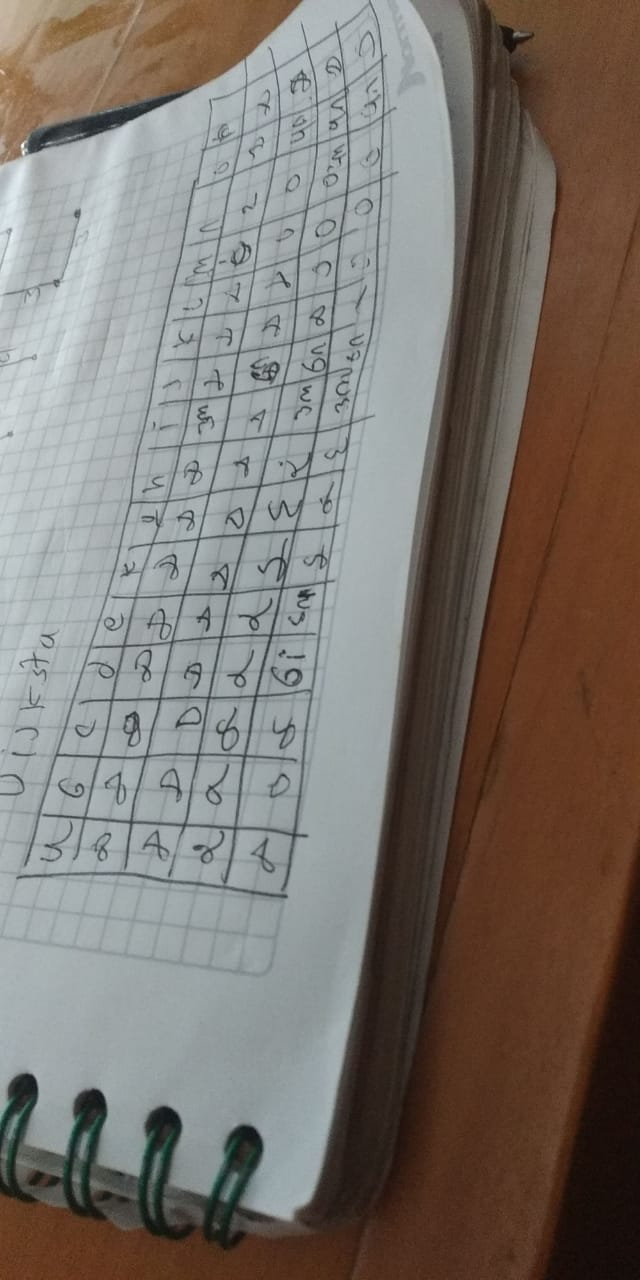
\includegraphics[width=0.4\linewidth]{tabladij.jpeg}
                \caption{primera parte tabla proceidmiento Dijkstra}
                \label{fig}
            \end{figure}




            % ====|ACA TERMINA EL PUNTO Dijkstra|==== %
    \newpage
    \section{Punto3}
        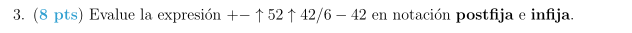
\includegraphics[width=0.8\linewidth]{postfi.png}

    \newpage
    \section{Punto4}
        \textbf{Emparejamiento máximo:}
        \\
        % ====|ACA EMPIEZA EL PUNTO emparejamiento maximo|====
            \begin{figure}[ht]
                \centering
                \incfig{emparejamientomax}
                \caption{emparejamiento maximo}
                \label{fig:emparejamientomax}
            \end{figure}



        % ====|ACA TERMINA EL PUNTO emparejamiento maximo|==== %
        \textbf{conjunto independiente máximo:}
        \\
        % ====|ACA EMPIEZA EL PUNTO Conjunto independiente maximo|====
            \begin{figure}[ht]
                \centering
                \incfig{conjuntomax}
                \caption{conjunto independiente maximo}
                \label{fig:conjuntomax}
            \end{figure}



        % ====|ACA TERMINA EL PUNTO Conjunto independiente maximo|==== %























    %=======================NOTES ENDS HERE===================%

    % bib stuff
    \nocite{*}
    \addtocontents{toc}{{}}
    \addcontentsline{toc}{section}{\refname}
    \bibliographystyle{plain}
    \bibliography{../Bibliography}
\end{document}
